\begin{figure}[h]
    \centering
    \begin{subfigure}[b]{0.4\textwidth}
        % Single MPS tensor
        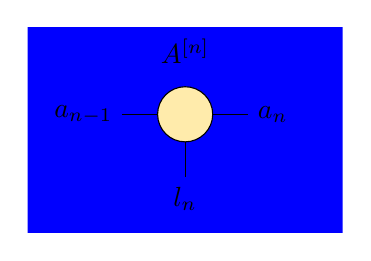
\begin{tikzpicture}
            \clip (-2,-1.5) rectangle (2, 1.1);
            \node[draw, shape=rectangle, fill=blue, minimum width=100cm, minimum height=100cm] (bg) at (0, 0) {};
            \definecolor{Tcolor}{RGB}{255, 235, 171}
            \def\textoffsetVertical{0.8}
            \def\nodewidth{0.7cm}
            \def\legwidth{0.8}
            \node[draw, shape=circle, fill=Tcolor, minimum width=\nodewidth] (T1) at (0, 0) {};
            \node[] (text1) at (0, \textoffsetVertical) {$A^{[n]}$};
            \draw (T1) -- ++(-\legwidth, 0);
            \draw (T1) -- ++(0, -\legwidth);
            \draw (T1) -- ++(\legwidth, 0);
            \node[anchor=east] at (-\legwidth, 0) {$a_{n-1}$};
            \node[anchor=west] at (+\legwidth, 0) {$a_{n}$};
            \node[anchor=north] at (0, -\legwidth) {$l_{n}$};
        \end{tikzpicture}
    \end{subfigure}
    \begin{subfigure}[b]{0.4\textwidth}
        % MPS
        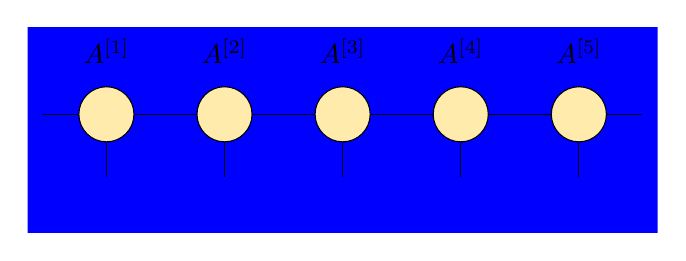
\begin{tikzpicture}
            \definecolor{Tcolor}{RGB}{255, 235, 171}
            \def\textoffsetVertical{0.8}
            \def\nodewidth{0.7cm}
            \def\legwidth{0.8}
            \def\nodedistance{1.5}
            \clip (-1,-1.5) rectangle ({4*\nodedistance+1}, 1.1);
            \node[draw, shape=rectangle, fill=blue, minimum width=100cm, minimum height=100cm] (bg )at (0, 0) {};
            \node[draw, shape=circle, fill=Tcolor, minimum width=\nodewidth] (T1) at (0, 0) {};
            \node[] (text1) at (0, \textoffsetVertical) {$A^{[1]}$};
            \node[draw, shape=circle, fill=Tcolor, minimum width=\nodewidth] (T2) at (\nodedistance, 0) {};
            \node[] (text1) at (\nodedistance, \textoffsetVertical) {$A^{[2]}$};
            \node[draw, shape=circle, fill=Tcolor, minimum width=\nodewidth] (T3) at ({2*\nodedistance}, 0) {};
            \node[] (text1) at ({2*\nodedistance}, \textoffsetVertical) {$A^{[3]}$};
            \node[draw, shape=circle, fill=Tcolor, minimum width=\nodewidth] (T4) at ({3*\nodedistance}, 0) {};
            \node[] (text1) at ({3*\nodedistance}, \textoffsetVertical) {$A^{[4]}$};
            \node[draw, shape=circle, fill=Tcolor, minimum width=\nodewidth] (T5) at ({4*\nodedistance}, 0) {};
            \node[] (text1) at ({4*\nodedistance}, \textoffsetVertical) {$A^{[5]}$};
            \draw (T1) -- (T2) -- (T3) -- (T4) -- (T5) -- ++(\legwidth, 0);
            \draw (T1) -- ++(-\legwidth, 0);
            \draw (T1) -- ++(0, -\legwidth);
            \draw (T2) -- ++(0, -\legwidth);
            \draw (T3) -- ++(0, -\legwidth);
            \draw (T4) -- ++(0, -\legwidth);
            \draw (T5) -- ++(0, -\legwidth);
        \end{tikzpicture}
    \end{subfigure}
    \begin{subfigure}[b]{0.4\textwidth}
        % Single MPO tensor
        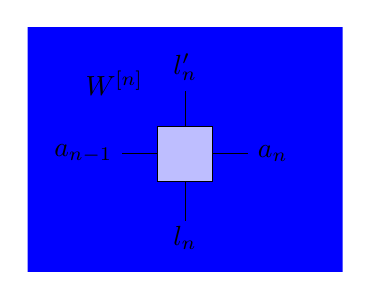
\begin{tikzpicture}
            \clip (-2,-1.5) rectangle (2, 1.6);
            \node[draw, shape=rectangle, fill=blue, minimum width=100cm, minimum height=100cm] (bg) at (0, 0) {};
            \definecolor{Tcolor}{RGB}{190, 190, 255}
            \def\textoffsetVertical{0.9}
            \def\textoffsetHorizontal{-0.9}
            \def\nodewidth{0.7cm}
            \def\legwidth{0.8}
            \node[draw, shape=rectangle, fill=Tcolor, minimum width=\nodewidth, minimum height=\nodewidth] (T1) at (0, 0) {};
            \node[] (text1) at (\textoffsetHorizontal, \textoffsetVertical) {$W^{[n]}$};
            \draw (T1) -- ++(-\legwidth, 0);
            \draw (T1) -- ++(0, -\legwidth5);
            \draw (T1) -- ++(\legwidth, 0);
            \draw (T1) -- ++(0, \legwidth);
            \node[anchor=east] at (-\legwidth, 0) {$a_{n-1}$};
            \node[anchor=west] at (+\legwidth, 0) {$a_{n}$};
            \node[anchor=north] at (0, -\legwidth) {$l_{n}$};
            \node[anchor=south] at (0, +\legwidth) {$l_{n}^\prime$};
        \end{tikzpicture}
    \end{subfigure}
    \begin{subfigure}[b]{0.4\textwidth}
        % MPO
        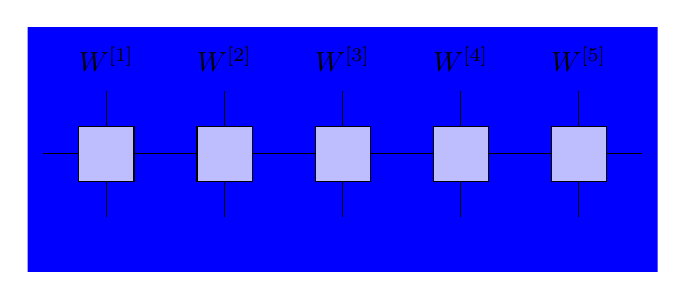
\begin{tikzpicture}
            \definecolor{Tcolor}{RGB}{190, 190, 255}
            \def\textoffsetVertical{1.2}
            \def\textoffsetHorizontal{-0.7}
            \def\nodewidth{0.7cm}
            \def\legwidth{0.8}
            \def\nodedistance{1.5}
            \clip (-1,-1.5) rectangle ({4*\nodedistance+1}, 1.6);
            \node[draw, shape=rectangle, fill=blue, minimum width=100cm, minimum height=100cm] (bg) at (0, 0) {};
            \node[] (text1) at (0, \textoffsetVertical) {$W^{[1]}$};
            \node[draw, shape=rectangle, fill=Tcolor, minimum width=\nodewidth, minimum height=\nodewidth] (T1) at (0, 0) {};
            \node[] (text1) at (\nodedistance, \textoffsetVertical) {$W^{[2]}$};
            \node[draw, shape=rectangle, fill=Tcolor, minimum width=\nodewidth, minimum height=\nodewidth] (T2) at (\nodedistance, 0) {};
            \node[] (text1) at ({2*\nodedistance}, \textoffsetVertical) {$W^{[3]}$};
            \node[draw, shape=rectangle, fill=Tcolor, minimum width=\nodewidth, minimum height=\nodewidth] (T3) at ({2*\nodedistance}, 0) {};
            \node[] (text1) at ({3*\nodedistance}, \textoffsetVertical) {$W^{[4]}$};
            \node[draw, shape=rectangle, fill=Tcolor, minimum width=\nodewidth, minimum height=\nodewidth] (T4) at ({3*\nodedistance}, 0) {};
            \node[] (text1) at ({4*\nodedistance}, \textoffsetVertical) {$W^{[5]}$};
            \node[draw, shape=rectangle, fill=Tcolor, minimum width=\nodewidth, minimum height=\nodewidth] (T5) at ({4*\nodedistance}, 0) {};
            \draw (T1) -- (T2) -- (T3) -- (T4) -- (T5) -- ++(\legwidth, 0);
            \draw (T1) -- ++(-\legwidth, 0);
            \draw (T1) -- ++(0, -\legwidth);
            \draw (T2) -- ++(0, -\legwidth);
            \draw (T3) -- ++(0, -\legwidth);
            \draw (T4) -- ++(0, -\legwidth);
            \draw (T5) -- ++(0, -\legwidth);
            \draw (T1) -- ++(0, \legwidth);
            \draw (T2) -- ++(0, \legwidth);
            \draw (T3) -- ++(0, \legwidth);
            \draw (T4) -- ++(0, \legwidth);
            \draw (T5) -- ++(0, \legwidth);
        \end{tikzpicture}
    \end{subfigure}
    \centering
    \begin{subfigure}[b]{\textwidth}
        % MPO applied to MPS
        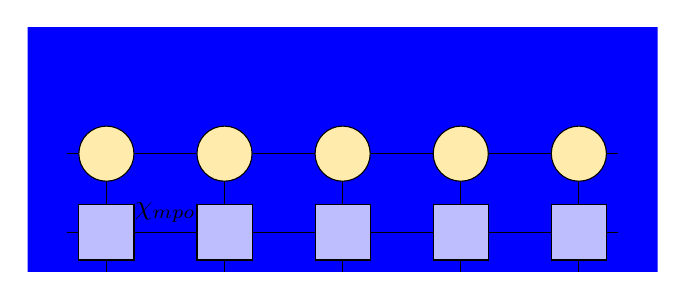
\begin{tikzpicture}
            \definecolor{Tcolor}{RGB}{255, 235, 171}
            \definecolor{Wcolor}{RGB}{190, 190, 255}
            \def\nodewidth{0.7cm}
            \def\legwidth{0.8}
            \def\nodedistance{1.5}
            \def\yoffset{1}
            \clip (-1,-1.5) rectangle ({4*\nodedistance+1}, 1.6);
            \node[draw, shape=rectangle, fill=blue, minimum width=100cm, minimum height=100cm] (bg) at (0, 0) {};
            % MPS
            \node[draw, shape=circle, fill=Tcolor, minimum width=\nodewidth] (T1) at (0, 0) {};
            \node[draw, shape=circle, fill=Tcolor, minimum width=\nodewidth] (T2) at (\nodedistance, 0) {};
            \node[draw, shape=circle, fill=Tcolor, minimum width=\nodewidth] (T3) at ({2*\nodedistance}, 0) {};
            \node[draw, shape=circle, fill=Tcolor, minimum width=\nodewidth] (T4) at ({3*\nodedistance}, 0) {};
            \node[draw, shape=circle, fill=Tcolor, minimum width=\nodewidth] (T5) at ({4*\nodedistance}, 0) {};
            \draw (T1) -- (T2) -- (T3) -- (T4) -- (T5) -- ++(0.5, 0);
            \draw (T1) -- ++(-0.5, 0);
            % MPO
            \node[draw, shape=rectangle, fill=Wcolor, minimum width=\nodewidth, minimum height=\nodewidth] (W1) at (0, -\yoffset) {};
            \node[draw, shape=rectangle, fill=Wcolor, minimum width=\nodewidth, minimum height=\nodewidth] (W2) at (\nodedistance, -\yoffset) {};
            \node[draw, shape=rectangle, fill=Wcolor, minimum width=\nodewidth, minimum height=\nodewidth] (W3) at ({2*\nodedistance}, -\yoffset) {};
            \node[draw, shape=rectangle, fill=Wcolor, minimum width=\nodewidth, minimum height=\nodewidth] (W4) at ({3*\nodedistance}, -\yoffset) {};
            \node[draw, shape=rectangle, fill=Wcolor, minimum width=\nodewidth, minimum height=\nodewidth] (W5) at ({4*\nodedistance}, -\yoffset) {};
            \draw (W1) -- node[midway,above] {$\chi_{mpo}$} (W2) -- (W3) -- (W4) -- (W5) -- ++(0.5, 0);
            \draw (T1) -- (W1);
            \draw (T2) -- (W2);
            \draw (T3) -- (W3);
            \draw (T4) -- (W4);
            \draw (T5) -- (W5);
            \draw (W1) -- ++(-0.5, 0);
            \draw (W1) -- ++(0, -0.5);
            \draw (W2) -- ++(0, -0.5);
            \draw (W3) -- ++(0, -0.5);
            \draw (W4) -- ++(0, -0.5);
            \draw (W5) -- ++(0, -0.5);
        \end{tikzpicture}
    \end{subfigure}
\end{figure}

\iffalse
% MPO applied to an MPS
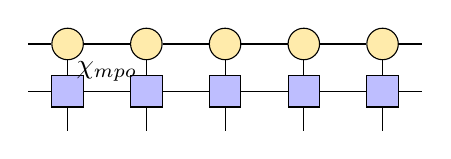
\begin{tikzpicture}
    \definecolor{Tcolor}{RGB}{255, 235, 171}
    \definecolor{Wcolor}{RGB}{190, 190, 255}
    \def\nodewidth{0.4cm}
    \def\yoffset{0.6}
    % MPS
    \node[draw, shape=circle, fill=Tcolor, minimum width=\nodewidth] (T1) at (0, 0) {};
    \node[draw, shape=circle, fill=Tcolor, minimum width=\nodewidth] (T2) at (1, 0) {};
    \node[draw, shape=circle, fill=Tcolor, minimum width=\nodewidth] (T3) at (2, 0) {};
    \node[draw, shape=circle, fill=Tcolor, minimum width=\nodewidth] (T4) at (3, 0) {};
    \node[draw, shape=circle, fill=Tcolor, minimum width=\nodewidth] (T5) at (4, 0) {};
    \draw (T1) -- (T2) -- (T3) -- (T4) -- (T5) -- ++(0.5, 0);
    \draw (T1) -- ++(-0.5, 0);
    % MPO
    \node[draw, shape=rectangle, fill=Wcolor, minimum width=\nodewidth, minimum height=\nodewidth] (W1) at (0, -\yoffset) {};
    \node[draw, shape=rectangle, fill=Wcolor, minimum width=\nodewidth, minimum height=\nodewidth] (W2) at (1, -\yoffset) {};
    \node[draw, shape=rectangle, fill=Wcolor, minimum width=\nodewidth, minimum height=\nodewidth] (W3) at (2, -\yoffset) {};
    \node[draw, shape=rectangle, fill=Wcolor, minimum width=\nodewidth, minimum height=\nodewidth] (W4) at (3, -\yoffset) {};
    \node[draw, shape=rectangle, fill=Wcolor, minimum width=\nodewidth, minimum height=\nodewidth] (W5) at (4, -\yoffset) {};
    \draw (W1) -- node[midway,above] {$\chi_{mpo}$} (W2) -- (W3) -- (W4) -- (W5) -- ++(0.5, 0);
    \draw (T1) -- (W1);
    \draw (T2) -- (W2);
    \draw (T3) -- (W3);
    \draw (T4) -- (W4);
    \draw (T5) -- (W5);
    \draw (W1) -- ++(-0.5, 0);
    \draw (W1) -- ++(0, -0.5);
    \draw (W2) -- ++(0, -0.5);
    \draw (W3) -- ++(0, -0.5);
    \draw (W4) -- ++(0, -0.5);
    \draw (W5) -- ++(0, -0.5);
\end{tikzpicture}
\end{document}
\fi